\chapter{Existence and Uniqueness of Solutions}

In this topic, we would like to address the existence and uniqueness to the general 
first-order IVP:

\begin{equation}
    y' = f(x,y), \quad y(x_0) = y_0
\end{equation}

\begin{theorem}[Peano's Existence theorem]
    Let $R = \{(x,y) \> | \> a < x < b, c < y < d \}$ be a open rectangular 
    region containing the point $(x_0, y_0)$. If the function $f(x, y)$ 
    is continuous in $R$.

    \[
        y' = f(x,y), \quad y(x_0) = y_0
    \]

    \begin{center}
    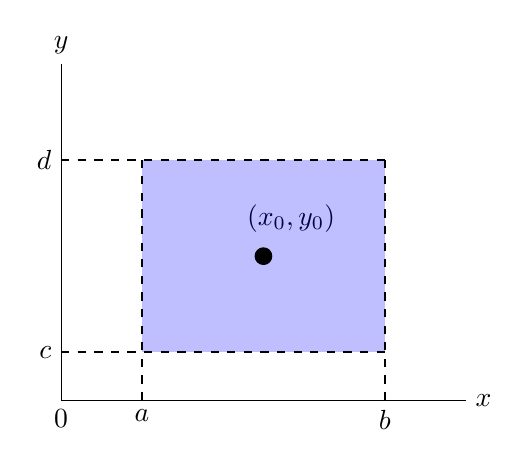
\begin{tikzpicture}
    \begin{axis}[
    scale = 0.75,
    xmin = 0, xmax = 10,
    ymin = 0, ymax = 7,
    axis lines* = left,
    xtick = {0}, ytick = \empty,
    clip = false,
    ]
    % Labels
    \node [right] at (current axis.right of origin) {$x$};
    \node [above] at (current axis.above origin) {$y$};
    \node [below] at (2, 0) {$a$};
    \node [below] at (8, 0) {$b$};
    \node [left] at (0, 1) {$c$};
    \node [left] at (0, 5) {$d$};
    
    % mark the centre of rectangle
    \addplot[color = black, mark = *, only marks, mark size = 3pt] coordinates {(5,3)};
    
    % labelling the centre of rectangle
    \node [right = 10pt, above = 5pt] at (5, 3) {$(x_0, y_0)$};

    % Colouring areas
    \fill[blue, opacity = 0.25] (2, 1)-- (2, 5) -- (8, 5) -- (8, 1);

    % Dashed lines (y-axis)
    \addplot[color = black, dashed, thick] coordinates {(0, 1) (8, 1)};
    \addplot[color = black, dashed, thick] coordinates {(0, 5) (8, 5)};

    % Dashed lines (x-axis)
    \addplot[color = black, dashed, thick] coordinates {(2, 0) (2, 5)};
    \addplot[color = black, dashed, thick] coordinates {(8, 0) (8, 5)};

    \end{axis}
    \end{tikzpicture}
\end{center}

    in some interval $x_0 - h < x < x_0 + h$ contained in $a < x < b$.
\end{theorem}

\begin{example}
    Determine whether Peano's Existence theorem does or does not guarantee existence of a 
    solution of the initial value problem:
    \[
        xy' = y,\quad y(1) = 0
    \]
\end{example}
\begin{solution}
    The DE can be written as $y' = f(x,y)$ where $ f(x,y) = \frac{y}{x}$. 
    Observe that $f$ is continuous everywhere in the $xy$-plane except on the line 
    $x = 0$ (which is the $y$-axis). Since the initial point $(1, 0)$. Hence,
    the theorem guarantees the existence of a solution of the IVP.
\end{solution}

The next example tells us that there are first-order initial value problems that have 
more than one solutions.

\newpage

\subsection*{An IVP with more than one solution}

\begin{example}
    Verify that the function $y_1 = 0$ and $y_2 = x$ are solutions of the initial value problem

    \[
        xy' = y,\quad y(0) = 0
    \]
\end{example}

\begin{remark}
    The function $f(x,y) = \frac{y}{x}$ is continuous everywhere in the plane except
    at the points $(x, y)$ where $x=0$. Thus, Peano Existence theorem does not guarantee 
    the existence of a solution in some neighbourhood of the initial point $(0,0)$.
\end{remark}

\begin{theorem}[Picard's Existence and Uniqueness Theorem]
    Let $R = \{(x,y) \> | \> a < x < b, c < y < d\}$ be an open rectangular region 
    containing the point $(x_0, y_0)$.
\end{theorem}

\begin{example}
    Determine whether Picard's theorem guarantees that the first-order IVP
    \[
        y' = y^2 + x^3, \quad y(2) = 5
    \]
    has a unique solution.
\end{example}
\begin{solution}
    Consider the following IVP

    \[
        \begin{cases}
            y' = f(x,y) = y^2 + x^3\\
            y(2) = 5
        \end{cases}
    \]

    Observe that $f$ is continuous $\forall (x,y) \in \mathbb{R}$. And since
    \[
        f_y(x, y) = \frac{\partial f}{\partial y}=2y \text{ is continuous } \forall (x,y) \in \mathbb{R}
    \]
    Thus, $f$ and $\frac{\partial f}{\partial y}$ are continuous near the initial point (2, 5). 
    By Picard's theorem, this IVP has a unique solution.
\end{solution}